\documentclass[12pt,a4paper]{article}
\usepackage[utf8]{inputenc}
\usepackage[spanish,es-tabla]{babel}
\usepackage{geometry}
\usepackage{graphicx}
\usepackage{multirow}
\usepackage{tabularx}
\usepackage{mathptmx}
\usepackage{fancyhdr}
\usepackage{array}
\usepackage[table]{xcolor}
\usepackage{titlesec}
\usepackage{setspace}
\usepackage{microtype}
\usepackage{lastpage}
\usepackage{booktabs}
\usepackage{enumitem}
\usepackage{amsmath}
\usepackage{amsfonts}
\usepackage{amssymb}

\graphicspath{{images/}{../images/}{./}}

\geometry{
    top=4.7cm,
    bottom=2.5cm,
    left=2.5cm,
    right=2.5cm,
    headheight=3.9cm,
    headsep=0.4cm
}

\setstretch{1.15}
\setlength{\parindent}{0pt}
\setlength{\parskip}{0.45em}
\setlength{\tabcolsep}{4pt}

\titleformat{\section}
  {\normalfont\fontsize{12}{14.5}\bfseries}{\thesection.}{0.6em}{\uppercase}
\titlespacing*{\section}
  {0pt}{1.8ex plus 0.4ex minus 0.2ex}{0.6ex plus 0.2ex}

\titleformat{\subsection}
  {\normalfont\fontsize{11.5}{13.5}\bfseries}{\thesubsection.}{0.5em}{}
\titlespacing*{\subsection}
  {0pt}{1.4ex plus 0.3ex minus 0.1ex}{0.4ex plus 0.1ex}

\titleformat{\subsubsection}
  {\normalfont\fontsize{10.5}{12.5}\bfseries\itshape}{\thesubsubsection.}{0.4em}{}
\titlespacing*{\subsubsection}
  {0pt}{1.1ex plus 0.2ex minus 0.1ex}{0.3ex plus 0.1ex}

\newcolumntype{Y}{>{\centering\arraybackslash}X}
\newcolumntype{L}{>{\raggedright\arraybackslash}X}
\newcolumntype{C}{>{\centering\arraybackslash}X}

\definecolor{headerblue}{RGB}{26, 54, 93}
\definecolor{darkblue}{RGB}{43, 108, 176}
\definecolor{lightgraybg}{RGB}{248, 248, 248}
\definecolor{tableheader}{RGB}{232, 238, 246}

\newcommand{\docCodigo}{TI-SIGE-ENT-F3-016}
\newcommand{\docVersion}{1.0}
\newcommand{\docProceso}{HITO DE CONTROL / CODE FREEZE FASE 3}
\newcommand{\docElaboracion}{08/10/2026}
\newcommand{\docRevision}{08/10/2026}
\newcommand{\docTitulo}{HITO 5: SISTEMA CORE COMPLETADO}
\newcommand{\docOrganizacion}{FACULTAD DE INGENIERÍA EN SISTEMAS, ELECTRÓNICA E INDUSTRIAL}
\newcommand{\docSubOrganizacion}{CARRERA DE INGENIERÍA DE SOFTWARE}

\newcommand{\encabezadofrecuente}{%
    \renewcommand{\arraystretch}{1.15}%
    \noindent\makebox[\textwidth][c]{%
    \begin{tabularx}{\textwidth}{|>{\centering\arraybackslash}m{2.8cm}|Y|>{\centering\arraybackslash}m{4.8cm}|}
        \hline
        \multirow{4}{2.8cm}{\centering\raisebox{-1.15cm}{
\includegraphics[width=2.5cm,height=2.0cm,keepaspectratio]{images/logo.png}}}
        & \textbf{\fontsize{9}{11}\selectfont \docOrganizacion} 
        & \textbf{\fontsize{8}{10}\selectfont CÓDIGO:} \fontsize{8}{10}\selectfont \docCodigo \\
        \cline{3-3}
        & \textbf{\fontsize{8.5}{10.5}\selectfont \docSubOrganizacion} 
        & \textbf{\fontsize{8}{10}\selectfont VERSIÓN:} \fontsize{8}{10}\selectfont \docVersion \\
        \cline{2-3}
        & \textbf{\fontsize{8}{10}\selectfont PROCESO:} \fontsize{8}{10}\selectfont \docProceso 
        & \textbf{\fontsize{8}{10}\selectfont ELABORACIÓN:} \fontsize{8}{10}\selectfont \docElaboracion \\
        \cline{2-3}
        & \textbf{\fontsize{8.5}{10.5}\selectfont \docTitulo} 
        & \textbf{\fontsize{8}{10}\selectfont ÚLTIMA REVISIÓN:} \fontsize{8}{10}\selectfont \docRevision \\
        \hline
    \end{tabularx}%
    }%
}

\pagestyle{fancy}
\fancyhf{}
\fancyhead[C]{\encabezadofrecuente}
\fancyfoot[C]{\fontsize{10}{12}\selectfont Página \thepage\ de \pageref{LastPage}}
\renewcommand{\headrulewidth}{0pt}

\begin{document}

\noindent{\fontsize{10.5}{12.5}\selectfont \textbf{Integrantes:} Heidi Villavicencio \quad$\vert$\quad Steeven Toala \quad$\vert$\quad Nixon Hurtado \quad$\vert$\quad Andrea Vásquez}

\vspace{0.25cm}

\section{Título}
\textbf{Denominación del Entregable:} HITO 5: Sistema Core Completado (Code Freeze) -- Código EDT: 3.16

\section{Introducción}
La culminación de la Fase 3: Desarrollo Core representa el logro técnico más trascendente del proyecto SIGE. A lo largo de 24 días laborables y 192 horas de desarrollo continuo (del 07 de septiembre al 08 de octubre de 2026), se implementó exitosamente el 100\% de las funcionalidades estipuladas en la especificación SRS IEEE 830. El presente informe formaliza la sesión de congelamiento de código (Code Freeze) ejecutada el jueves 08 de octubre de 2026, previo al feriado nacional del 9 de octubre (Independencia de Guayaquil). Se consolida la versión operativa v0.9 con el tag Git \texttt{v0.9-beta-freeze} y se autoriza el paso a la Fase 4 de Pruebas y Control de Calidad.

\section{Objetivo}
\subsection{Objetivo General}
Consolidar, evaluar y aprobar formalmente el Hito 5: Sistema Core Completado (Code Freeze), certificando la disponibilidad funcional del software para el inicio de la Fase 4 de Pruebas.
\subsection{Objetivos Específicos}
\begin{itemize}[leftmargin=1.5em, itemsep=2pt]
    \item Verificar el cumplimiento del 100\% de los 24 Requerimientos Funcionales (RF-01 a RF-24).
    \item Realizar el cierre y fusión formal de Pull Requests en la rama principal del repositorio Git.
    \item Generar la etiqueta de versión inmutable \texttt{v0.9-beta-freeze}.
    \item Suscribir el acta formal de aprobación de Hito 5 por parte del docente evaluador Ing. Paulo Torres.
\end{itemize}

\section{Alcance}
\subsection{Límites del Entregable (In-Scope)}
\begin{itemize}[leftmargin=1.5em, itemsep=2pt]
    \item Consolidado de los 16 entregables de Fase 3 ejecutados entre el 07 de septiembre y el 08 de octubre de 2026.
    \item Congelamiento de funcionalidades: no se añadirán nuevas características durante la Fase 4 de QA.
\end{itemize}
\subsection{Exclusiones (Out-of-Scope)}
\begin{itemize}[leftmargin=1.5em, itemsep=2pt]
    \item Reportes de pruebas de carga o pentesting (objeto de la Fase 4).
\end{itemize}

\section{Definiciones}
\begin{itemize}[leftmargin=1.5em, itemsep=2pt]
    \item \textbf{Code Freeze (Congelamiento de Código):} Punto en el ciclo de desarrollo donde se suspende estrictamente la adición de nuevas funcionalidades para permitir un ciclo riguroso de pruebas y estabilización.
    \item \textbf{Release Tag:} Puntero inmutable en el historial de Git que marca una versión específica del código fuente.
    \item \textbf{Hito 5 (Sistema Core Completado):} Hito contractual que certifica que el software posee todas las capacidades requeridas por el usuario.
\end{itemize}

\section{Responsabilidades}
\begin{itemize}[leftmargin=1.5em, itemsep=2pt]
    \item \textbf{Equipo de Proyecto SIGE (Responsables EDT 3.16):} Cierre de ramas de desarrollo, empaquetado del tag Git y sustentación general.
    \item \textbf{Ing. Paulo Torres (Docente Evaluador / Patrocinador):} Revisión integral de cobertura, inspección del sistema y aprobación formal de cierre de Fase 3.
\end{itemize}

\section{Normativa Legal y Técnica}
\begin{itemize}[leftmargin=1.5em, itemsep=2pt]
    \item \textbf{IEEE Std 1074-2006:} Standard for Developing a Software Project Life Cycle Process.
    \item \textbf{Guía PMBOK (7ma Edición):} Gestión de la Calidad y Aprobación de Entregables Principales.
\end{itemize}

\section{Método, Políticas y Contenidos}
Se realizó una sesión técnica de Code Freeze y sustentación de 90 minutos el 08 de octubre de 2026. En la Figura \ref{fig:f3_16_core} se ilustra el tablero consolidado de avance del proyecto.

\begin{figure}[htbp]
    \centering
    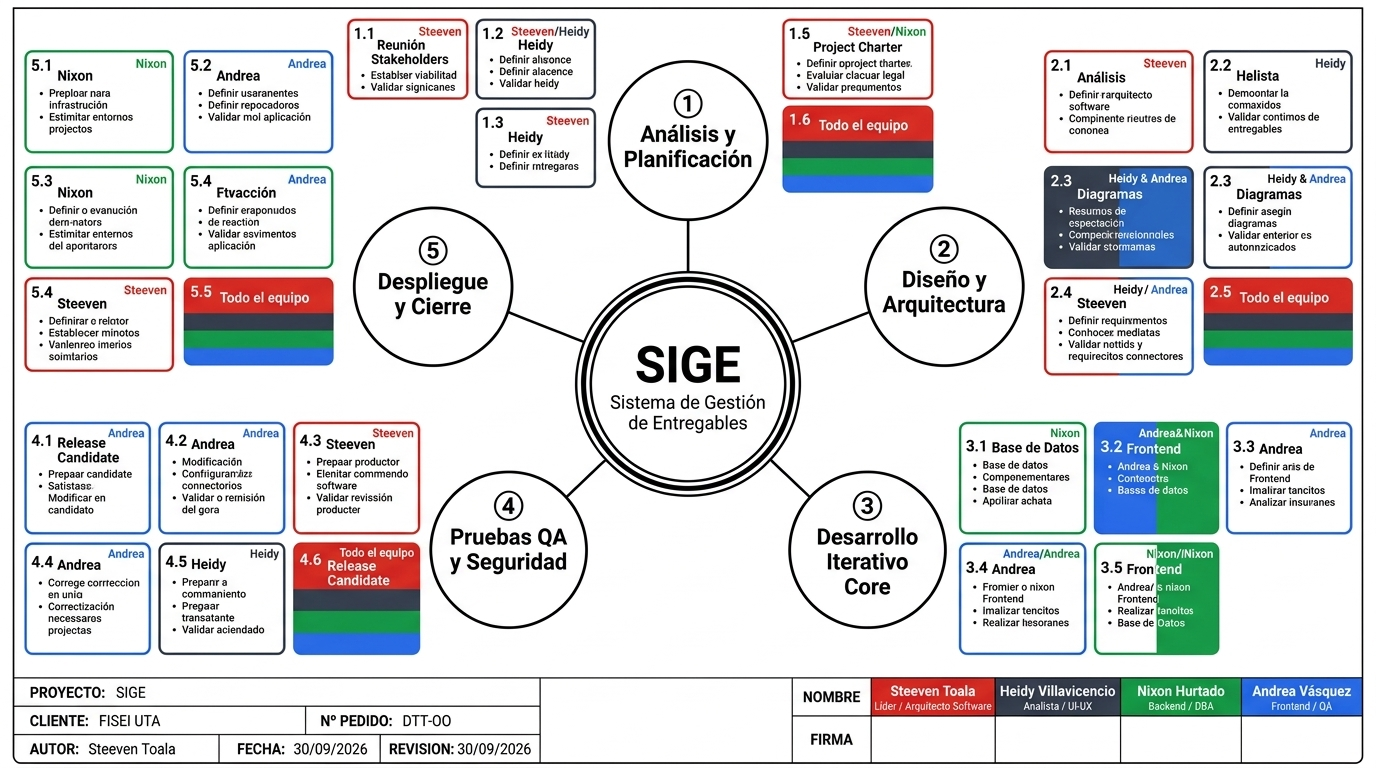
\includegraphics[width=0.88\textwidth,height=5.2cm,keepaspectratio]{images/trello_tablero_fases.jpg}
    \caption{Tablero de Control del Proyecto SIGE con Fase 3 Core Culminada al 100\%.}
    \label{fig:f3_16_core}
\end{figure}

\section{Descripción de actividades}
\subsection{Matriz de Cumplimiento de Requerimientos Funcionales en Fase 3}
\begin{table}[htbp]
\centering
\small
\renewcommand{\arraystretch}{1.2}
\begin{tabularx}{\textwidth}{|c|>{\bfseries}m{4.0cm}|X|c|c|}
\hline
\rowcolor{tableheader}
\textbf{Módulo} & \textbf{Requerimientos SRS} & \textbf{Componentes Implementados} & \textbf{Horas} & \textbf{Estado} \\
\hline
Base de Datos & RF-01, RF-02, RF-23 & 13 tablas relacionales DDL y catálogos en PostgreSQL 18 & 56 h & Aprobado \\
\hline
Seguridad & RF-01, RF-02 & JWT Auth, bcrypt y middlewares RBAC & 32 h & Aprobado \\
\hline
Frontend & RF-03 a RF-06 & SPA React + Vite, Wizard de 4 pasos y Editor TipTap & 104 h & Aprobado \\
\hline
Matriz \& Gates & RF-07 a RF-09, RF-13, 14 & Matriz interactiva reactiva y Validation Gates en Express & 80 h & Aprobado \\
\hline
Storage & RF-10 a RF-12 & Custodia MinIO S3 con hashes SHA-256 inmutables & 32 h & Aprobado \\
\hline
Comité \& Firmas & RF-15 a RF-18 & Panel de Comité, observaciones y Cascada de 3 firmas & 40 h & Aprobado \\
\hline
Asistencia & RF-19, RF-20 & Microservicio LanguageTool local y Google Gemini API & 32 h & Aprobado \\
\hline
Exportación & RF-21, RF-22 & Motor de salida idéntica SGC en PDF y Word con QR & 32 h & Aprobado \\
\hline
\multicolumn{3}{|r|}{\textbf{TOTAL HORAS INVERTIDAS EN FASE 3:}} & \textbf{192 h} & \textbf{100\%} \\
\hline
\end{tabularx}
\caption{Balance de Cobertura Funcional y Cierre de la Fase 3: Desarrollo Core.}
\label{tab:cierre_fase3}
\end{table}

\subsection{Acta de Declaración de Code Freeze y Paso a Fase 4}
El docente evaluador Ing. Paulo Torres certifica la culminación satisfactoria del Sistema Core en su versión v0.9, autorizando el inicio inmediato de la Fase 4 de Pruebas y Control de Calidad a partir del lunes 12 de octubre de 2026.

\section{Firmas de Responsabilidad}

\noindent
\renewcommand{\arraystretch}{1.2}
\begin{tabularx}{\textwidth}{|>{\raggedright\arraybackslash}m{2.9cm}|>{\raggedright\arraybackslash}X|>{\centering\arraybackslash}m{4.6cm}|>{\centering\arraybackslash}m{2.3cm}|}
    \hline
    \rowcolor{tableheader}
    \textbf{ACCIÓN} & \textbf{NOMBRE Y CARGO} & \textbf{FIRMA} & \textbf{FECHA} \\
    \hline
    \textbf{Elaborado por:} & Heidi Villavicencio\newline Analista de Calidad / UI-UX & \parbox[c]{4.4cm}{\centering\vspace{4pt}
\includegraphics[height=1.5cm,width=4.0cm,keepaspectratio]{images/firma_heidi.png}\vspace{4pt}} & 08/10/2026 \\
    \hline
    \textbf{Revisado por:} & Steeven Toala\newline Líder de Proyecto / Arquitecto & \parbox[c]{4.4cm}{\centering\vspace{4pt}
\includegraphics[height=1.5cm,width=4.0cm,keepaspectratio]{images/firma_steveen.png}\vspace{4pt}} & 08/10/2026 \\
    \hline
    \textbf{Aprobado por:} & Ing. Paulo Torres, Mg.\newline Docente Evaluador -- Gestión Proyectos & \parbox[c]{4.4cm}{\centering\vspace{8pt}\textbf{\textcolor{gray!80}{\scriptsize [ PENDIENTE DE APROBACIÓN ]}}\vspace{8pt}} & \textbf{\textcolor{gray!90}{Pendiente}} \\
    \hline
\end{tabularx}

\vspace{0.4cm}

\section{Control de Cambios}

\noindent
\renewcommand{\arraystretch}{1.2}
\begin{tabularx}{\textwidth}{|>{\hsize=0.45\hsize\centering\arraybackslash}X|>{\hsize=1.55\hsize\raggedright\arraybackslash}X|>{\hsize=1.2\hsize\raggedright\arraybackslash}X|>{\hsize=0.8\hsize\centering\arraybackslash}X|}
    \hline
    \rowcolor{tableheader}
    \textbf{Versión} & \textbf{Descripción del cambio} & \textbf{Responsable del cambio} & \textbf{Fecha de aprobación} \\
    \hline
    1.0 & Emisión inicial del entregable según EDT del Tablero Trello & Equipo de Proyecto SIGE & 08/10/2026 \\
    \hline
\end{tabularx}

\vspace{0.4cm}

\section{Anexos}
\begin{itemize}[leftmargin=1.5em]
\item \textbf{Anexo 1:} Acta Formal de Congelamiento de Código (Code Freeze).
\item \textbf{Anexo 2:} Registro del Tag Git \texttt{v0.9-beta-freeze} en el Repositorio Oficial.
\end{itemize}

\end{document}
